\chapter{Representation changes with learning}

To measure how the time representation changes with learning, we will compare the neural activity extracted from distinct learning stages. Specifically, we divide into the first and second half of the session for the group with long sessions, and into the first and second sessions for the group with short sessions. This is because for the first group we had long sessions of more than 1000 trials $(1149 \pm 384)$ with sufficient correct trials $(660 \pm 260)$. For the second group of animals, in which sessions were half as long with $570 \pm 181$ trials, there were only and $284\pm 100$ correct trials, less than half compared to the first group.

We will measure the quality of time representation using the same machine learning regression technique from the previous chapter. The number of neurons used in each group and each area was the same, and was kept constant in the multiple learning stages.

\section{Striatum enhances its representation while mPFC decreases}

\begin{figure}[ht]
    \centering
    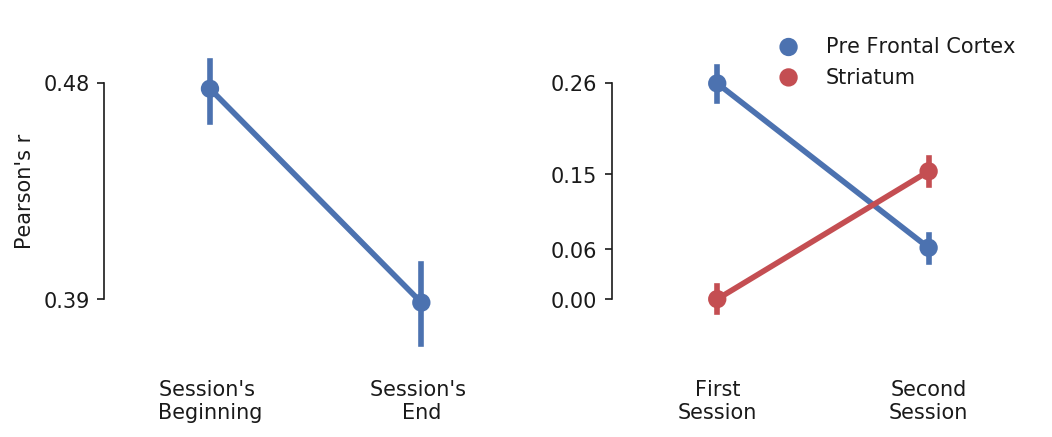
\includegraphics[width=\textwidth]{figures/pearson_comparison_before_after_learning.png}
    \caption[Comparison of classifier performances in distinct learning stages, by Pearson Correlation]{Comparison of classifier performances in distinct learning stages, by Pearson Correlation. Left: Group 1 at first half vs second half of session. Right: Group 2, in the first vs the second smaller sessions. In the vertical, we show the performance of the classifier as measured by Pearson's r. Values shown in the vertical axes correspond to the mean values of data points, shown as circles. The analysis was repeated 100 times, and error bars correspond to the confidence intervals of 95\% calculated by 1000 bootstrap averages of 100 samples with replacement.}
    \label{fig:evolution_representation_pearson}
\end{figure}

\begin{figure}[ht]
    \centering
    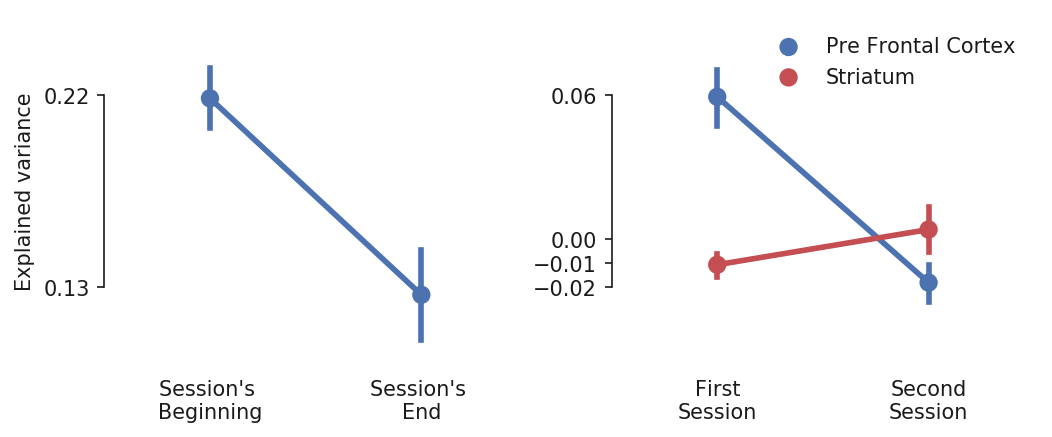
\includegraphics[width=\textwidth]{figures/expvar_comparison_before_after_learning.png}
    \caption[Comparison of classifier performances in distinct learning stages, by Explained variance]{Comparison of classifier performances in distinct learning stages, by Explained variance. Left: Group 1 at first half vs second half of session. Right: Group 2, in the first vs the second smaller sessions. In the vertical, we show the performance of the classifier as measured by Pearson's r. Values shown in the vertical axes correspond to the mean values of data points, shown as circles. The analysis was repeated 100 times, and error bars correspond to the confidence intervals of 95\% calculated by 1000 bootstrap averages of 100 samples with replacement.}
    \label{fig:evolution_representation_variance}
\end{figure}


When we compare the performance of classifiers as measured by Pearson correlation (figure \ref{fig:evolution_representation_pearson}), we see opposite trends for the two recorded areas. Performance in the mPFC decreases in both groups, while in the second group performance in the Striatum increases. The same pattern can be found in \ref{fig:evolution_representation_variance}, when measuring the same results with the explained variance metric. The main distinction between the results from each metric resides in the second session of the striatum, that is closer in value to the second session for the mPFC. All the distinctions between learning stages are statistically significant, shown in table \ref{tab:statistics_learning_stage}. 

In terms of Pearson's r, the only data in which the regression had null performance was the first session of the Striatum, in \ref{fig:evolution_representation_pearson}. If we look at the prediction distribution in \ref{fig:evolution_representation_density}, it is possible to see that the predictions are very close to a horizontal line, similar to the shuffled data. Differently, in the second session the distribution shows positive inclination, consistent with the increase in Pearson's r score.

The explained variance was null or negative in both sessions for the striatum

Medial Pre Frontal Cortex decreased its inclination


\begin{table}[ht]
    \centering
    \begin{tabular}{l|c|c|c}
        \hline
        Subjects & \multicolumn{1}{1}{Group 1} & \multicolumn{2}{1}{Group 2}\\
        Area & mPFC & mPFC & Striatum \\
        \hline
        Pearson's r         & $-8.19 \quad 10^{-12}$ 
                            & $-14.50 \quad 10^{-26}$ 
                            & $12.15 \quad 10^{-21}$ \\
        Explained variance  & $-7.33 \quad 10^{-11}$ 
                            & $-10.84 \quad 10^{-18}$ 
                            & $2.47 \quad .01$\\
        \hline
    \end{tabular}
    \caption[Significance of changes in decoder performance between training stages]{Significance of changes in decoder performance between training stages. We applied paired-sample T tests to compare each pair of training stages for each area recorded. Tests are shown for both Explained variance and Pearson's r metrics. In each cell, we have the t-value at left and the p-value at right. Values below .05 are considered statistically significant. Positive t-values indicate increase in the second stage with comparison to the first, and negative t-values indicate decrease.}
    \label{tab:statistics_learning_stage}
\end{table}

\begin{figure}[ht]
    \centering
    \begin{tabular}{cc}
    {\Large \qquad First Session}& {\Large \qquad Second Session}    \\\\
    
    \multicolumn{2}{1}{{\large Striatum}}\\\\
    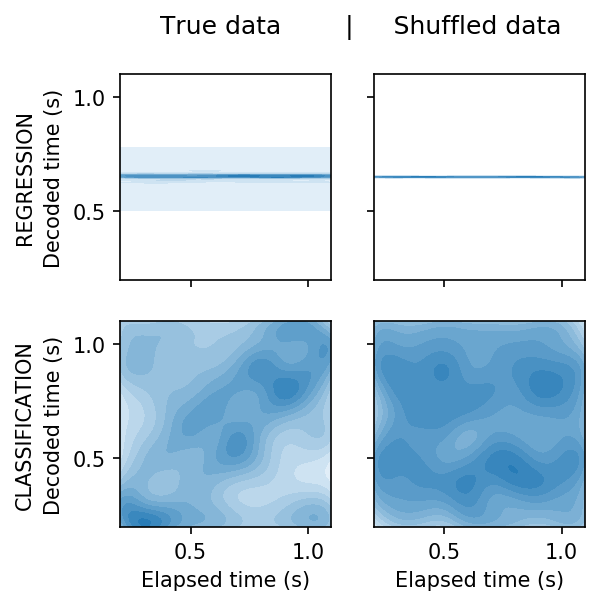
\includegraphics[width=0.45\textwidth]{figures/striatum_kde_bootstrap_vs_true_day1.png}    &  
    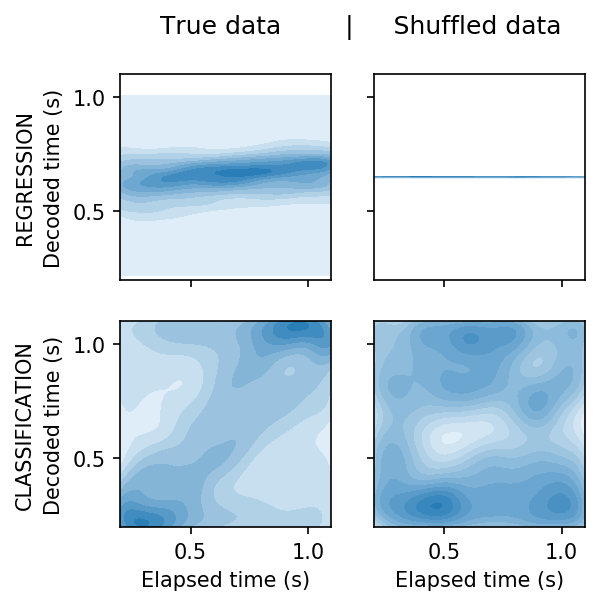
\includegraphics[width=0.45\textwidth]{figures/striatum_kde_bootstrap_vs_true_day2.png}    \\\\
    
    \multicolumn{2}{1}{{\large medial Pre Frontal Cortex}}\\\\
    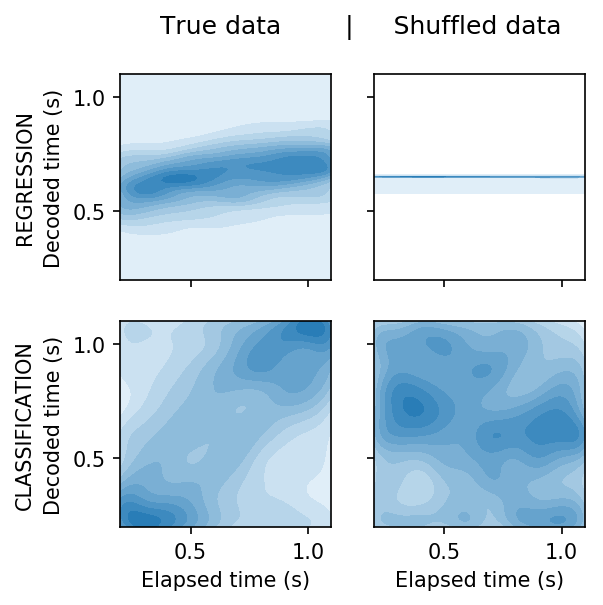
\includegraphics[width=0.45\textwidth]{figures/mpfc_kde_bootstrap_vs_true_day1.png}    &  
    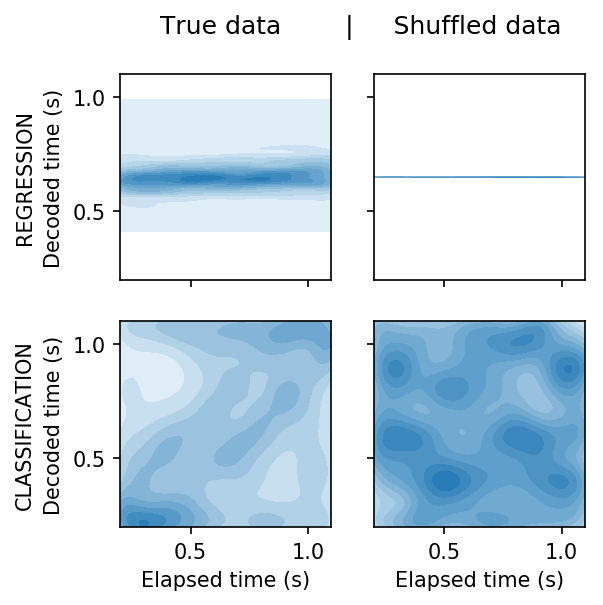
\includegraphics[width=0.45\textwidth]{figures/mpfc_kde_bootstrap_vs_true_day2.png}\\
    \end{tabular}
    \caption[Prediction density plots in the first vs second sessions]{Darker blues indicate higher density of points. For a given elapsed time, the vertical upon it is the distribution of all predictions calculated over neural activity extracted at that time.}
    \label{fig:evolution_representation_density}
\end{figure}